	%!TEX program = xelatex
	\documentclass{beamer}

	\usepackage{blindtext}

	\usetheme{FeecBUT}

	\usepackage{xltxtra}
	\usepackage{wrapfig}

	\defaultfontfeatures{Ligatures=TeX}

	\newcommand{\zdroj}[1]{\textcolor{ExecusharesGrey}{\tiny\hspace{1em} #1}}

	\title{Materiál GoreTex}
	\subtitle{MNAN 2016}
	\author{Martin Sehnoutka, Vojtěch Vladyka, Jan Žlebek}
	%\garant{Supervisor}
	\date{17. února, 2016}

	\begin{document}

	  \frame{\titlepage}
	   
	  \begin{frame}
		\frametitle{Obsah}
		\begin{enumerate}
		  \item Struktura materiálu
		  \\ \textcolor{ExecusharesGrey}{\footnotesize\hspace{1em} Chemické složení, výroba}	
		  \item Použití - oblečení, obuv
		  \\ \textcolor{ExecusharesGrey}{\footnotesize\hspace{1em} Nepromokavé membrány}
		  \item Použití - medicína
		  \\ \textcolor{ExecusharesGrey}{\footnotesize\hspace{1em} Inertní tkanina}
		\end{enumerate}
		\end{frame}
		
		\section{Struktura materiálu}
	
		\begin{frame}
			\frametitle{Co se skrývá pod názvem Gore-Tex \textregistered }
			\begin{itemize}
			  \item Expandovaný polytetrafluorethylen (všeobecně znám pod obchodním názvem Teflon\textregistered)
			  % Takže natažená pánvička?
			  \item Zkratka (anglická): ePTFE %TODO: zkontrolovat je jen anglická?
			  \item Membrána se z PTFE získá rychlým trhem po zahřátí materiálu (odtud expandovaný, natažený)
			  
			\end{itemize}
			
			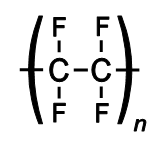
\includegraphics[width=0.2\textwidth]{Teflon_structure.PNG}
			
			\zdroj{GPL, https://commons.wikimedia.org/w/index.php?curid=839743}
			
		\end{frame}
		
		\begin{frame}
		  \frametitle{Historie}
		  \begin{itemize}
		    \item Vynálezci: Wilbert L. Gore a Robert W. Gore 
		    \item Rok: 1969
		  \end{itemize}
		\end{frame}
		
		\begin{frame}
		  \frametitle{Struktura}
		  \begin{itemize}
		    \item 
		  \end{itemize}
		  \begin{figure}
		    \begin{center}
		      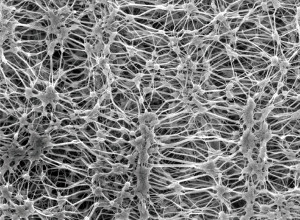
\includegraphics[width=200pt]{membrane_microscopy_small.jpg}
		      \caption{Membrána na snímku z elektronového mikroskopu}
		      \label{fig:membrana}
		    \end{center}
		  \end{figure}
		  \zdroj{http://www.evo.com/waterproof-ratings-and-breathability-guide.aspx}
		\end{frame}

		\section{Použití - oděvy, rukavice a obuv}

\begin{frame}
	\frametitle{Důvod}
	\begin{itemize}
		\item Nedostatečná nabídka voděodolných a zároveň prodyšných materiálů
		\item Původně určená pouze pro oděvy a stany
		\item Patent podán roku 1978 (US 4194041 A)
	\end{itemize}
\end{frame}

\begin{frame}
	\frametitle{Oděvy, rukavice a boty}
	\begin{itemize}
		\item Myšlenka materiálu: udržet vodu venku a zároveň nechat projít ven vlhkost
		\item Gore-Tex\textregistered nabízí 4 varianty konstrukce tkanin pro oděvy
		\begin{itemize}
			\item 2 vrstvá konstrukce % Out+gore, inner
			\item 3 vrstvá konstrukce % Out+gore+inner
			\item Z-liner konstrukce % Out, gore, inner
			\item LTD konstrukce % Out, gore+inner
		\end{itemize}
	  	\item V těchto konstrukcích se vyrábí kalohty a bundy.
	  	\item Rukavice mají navíc ještě tepelnou izolaci.
	\end{itemize}
\end{frame}

\begin{frame}
	\frametitle{2 vrstvá konstrukce}
			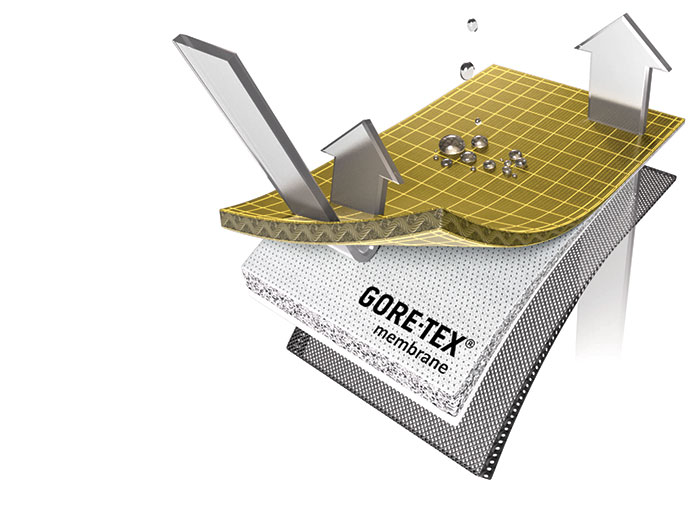
\includegraphics[width=0.8\textwidth]{bunda_close.jpg}
		\zdroj{http://www.gore-tex.com/en-us/technology/outerwear/gore-tex-products}
\end{frame}

\begin{frame}
	\frametitle{Konstrukce obuvi}
	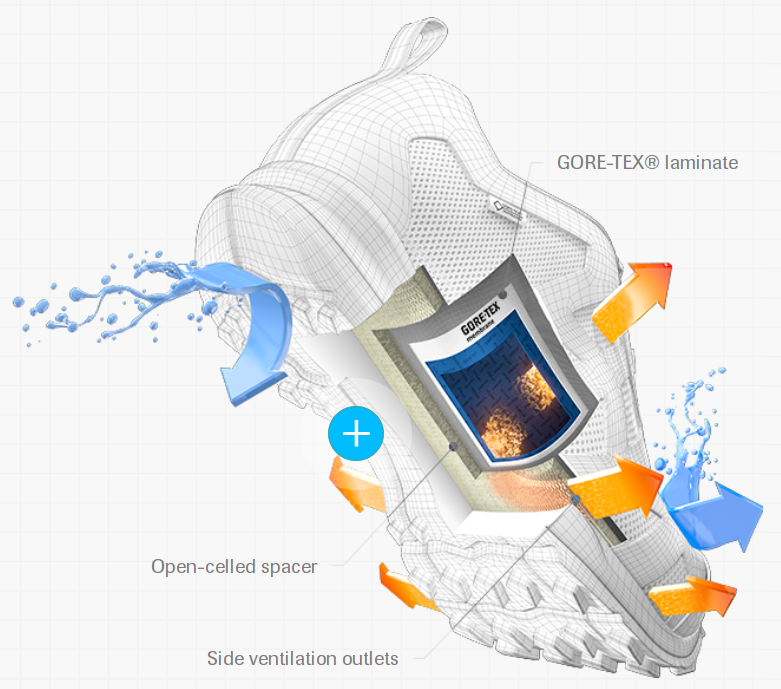
\includegraphics[width=0.65\textwidth]{bota_close.png}
	\zdroj{http://www.gore-tex.com/en-us/technology/footwear/gore-tex-surround-outdoor-footwear}
\end{frame}

		\section{Použití - medicína}

\begin{frame}
	\frametitle{Důležité vlastnosti}
	\begin{itemize}
		\item Nezpůsobuje alergické reakce
		\item V těle neprobíhají chemické reakce s tímto materiálem
		\item Nezpůsobuje záněty či šíření infekcí
		\item Bezpečné a pohodlné použití
	\end{itemize}
\end{frame}

\begin{frame}
	\frametitle{Cévní náhrady}
	\begin{itemize}
		\item Silný materiál
		\item Možnost pružné varianty
	\end{itemize}
	
\includegraphics[width=0.6\textwidth]{nahradni_ceva.jpg}
	\zdroj{http://www.goremedical.com/resources/images/popups/vgstretch.jpg}
\end{frame}

\begin{frame}
	\frametitle{Stehy}
	\begin{columns}
	\begin{column}{0.5\textwidth}
	\begin{itemize}
		\item Jemné, ohebné a pružné vlákno
		\item Nemá paměťový efekt
		\item Jehla stejně velká jako vlákno - zabraňuje úniku dírou po jehle 
	\end{itemize}
	\end{column}
	\begin{column}{0.5\textwidth}
		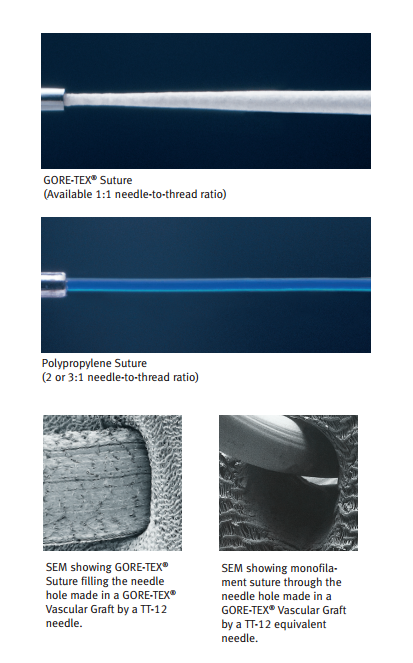
\includegraphics[scale=0.38]{needle_thread.png}
	\end{column}
	\end{columns}
	\zdroj{http://www.goremedical.com/resources/dam/assets/AB0101-EN6.pdf}
\end{frame}

\begin{frame}
	\frametitle{Další použití v medicíně}
	\begin{itemize}
		\item Operace trávicího traktu
		\item Operace srdce a plic
		\item Náhrada uložení páteřních cév
		\item Operace kýly
		\item Obecná chirurgie - záplaty, vlákna, ochrany
	\end{itemize}
\end{frame}

		\section{Dotazy?}
	
		\section{Děkujeme za pozornost}
	
\end{document}
